\let\negmedspace\undefined
\let\negthickspace\undefined
\documentclass[journal]{IEEEtran}
\usepackage[a5paper, margin=10mm, onecolumn]{geometry}
%\usepackage{lmodern} % Ensure lmodern is loaded for pdflatex
\usepackage{tfrupee} % Include tfrupee package

\setlength{\headheight}{1cm} % Set the height of the header box
\setlength{\headsep}{0mm}     % Set the distance between the header box and the top of the text

\usepackage{gvv-book}
\usepackage{gvv}
\usepackage{cite}
\usepackage{amsmath,amssymb,amsfonts,amsthm}
\usepackage{algorithmic}
\usepackage{graphicx}
\usepackage{textcomp}
\usepackage{xcolor}
\usepackage{txfonts}
\usepackage{listings}
\usepackage{enumitem}
\usepackage{mathtools}
\usepackage{gensymb}
\usepackage{comment}
\usepackage[breaklinks=true]{hyperref}
\usepackage{tkz-euclide} 
\usepackage{listings}
% \usepackage{gvv}                                        
\def\inputGnumericTable{}                                 
\usepackage[latin1]{inputenc}                                
\usepackage{color}                                            
\usepackage{array}                                            
\usepackage{longtable}                                       
\usepackage{calc}                                             
\usepackage{multirow}                                         
\usepackage{hhline}                                           
\usepackage{ifthen}                                           
\usepackage{lscape}
\begin{document}

\bibliographystyle{IEEEtran}
\vspace{3cm}

\title{1.2.26}
\author{AI24BTECH11036 - Shreedhanvi Yadlpally}

% \maketitle
% \newpage
% \bigskip
{\let\newpage\relax\maketitle}

\renewcommand{\thefigure}{\theenumi}
\renewcommand{\thetable}{\theenumi}
\setlength{\intextsep}{10pt} % Space between text and floats


\numberwithin{equation}{enumi}
\numberwithin{figure}{enumi}
\renewcommand{\thetable}{\theenumi}


\textbf{Question}:\\
A man can swim with a speed of 4.0 km/h in still water. How long does he take to cross a river 1.0 km wide if the river flows steadily at 3.0 km/h and he makes his strokes normal to the river current? How far down the river does he go when he reaches the outer bank? \\
\textbf{Solution: }
\begin{table}[h!]    
  \centering
  \begin{tabular}[12pt]{ |c| c|}
    \hline
    \textbf{Label} & \textbf{Co-ordinate}\\ 
    \hline
	\multicolumn{2}{|c|}{\textbf{Case (a)}}\\
	\hline
    $\vec{A}$ & $\brak{7, -2}$ \\
    \hline 
    $\vec{B}$ & $\brak{5, 1}$ \\
    \hline
    $\vec{C}$ & $\brak{3, k}$ \\
    \hline
	\multicolumn{2}{|c|} {\textbf{Case (b)}}\\
	\hline
    $\vec{A}$ & $\brak{8, 1}$ \\
    \hline 
    $\vec{B}$ & $\brak{k, -4}$ \\
    \hline
    $\vec{C}$ & $\brak{2, -5}$ \\
    \hline 
    \end{tabular}

  \caption{Variables Used}
  \label{tab 1.2.26.1}
\end{table}
\begin{align}
	v_{m} = 4.0 km/h \\
	v_{r} = 3.0 km/h \\
	w = 1.0 km
\end{align}
The man is swimming perpendicular to the river current, so his speed relative to the riverbank is 4.0 km/h (which is his speed in still water). Then,
\begin{align}
	t = \frac{w}{v_{m}} = \frac{1.0 km}{4.0 km/h} = 0.25 hours
\end{align}
For the distance he drifts downstream when he reaches the other bank,
\begin{align}
	d = v_{r} \times t = 3.0 km/h \times 0.25 hours = 0.75 km
\end{align}
For the resultant velocity vector
\begin{align}
	\vec{v_{m}}=\myvec{0 \\ 4} km/h \\
	\vec{v_{r}}=\myvec{3 \\ 0} km/h \\
	\vec{v_{res}}=\vec{v_{m}}+\vec{v_{r}}=\myvec{ 3 \\ 4} km/h
\end{align}
\begin{figure}[h!]
   \centering
   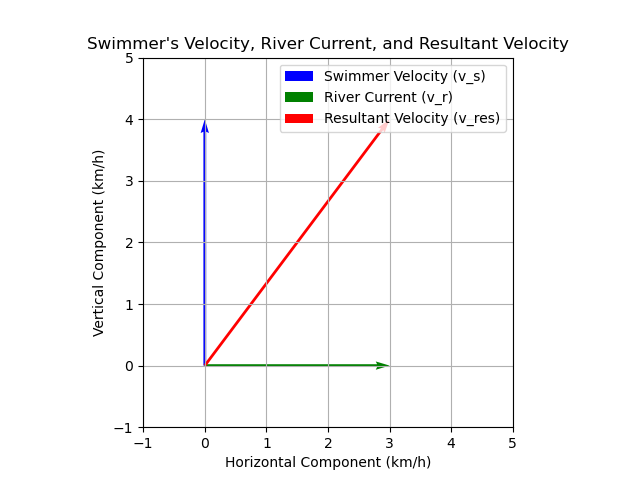
\includegraphics[width=0.7\linewidth]{figures/Figure_1.png}
   \caption{Vector Plot}
   \label{vector}
\end{figure}
\begin{figure}[h!]
   \centering
   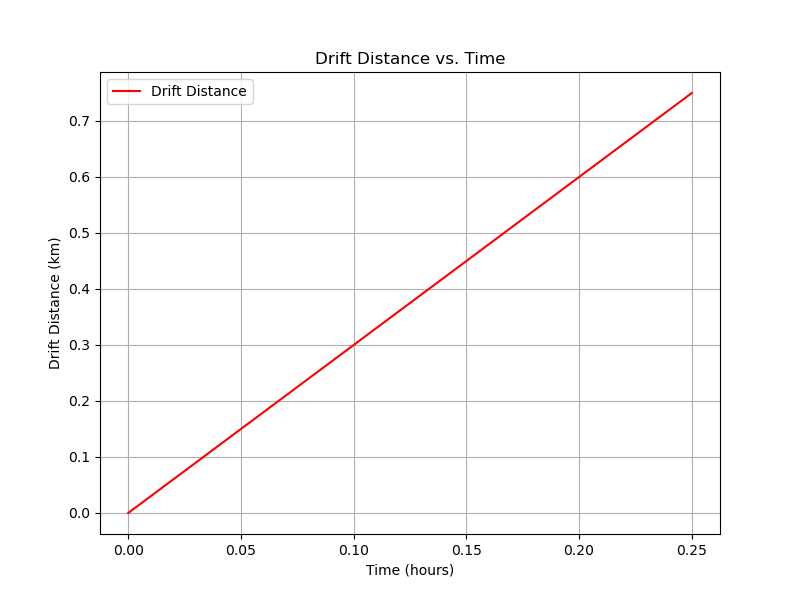
\includegraphics[width=0.7\linewidth]{figures/Figure_2.png}
   \label{graph}
\end{figure}


\end{document}



